\documentclass[11pt,a4paper]{article}

\usepackage[a4paper,margin=1in]{geometry}
\usepackage{graphicx}
\usepackage{booktabs}
\usepackage{tabularx}
\usepackage{array}
\usepackage{amsmath}
\usepackage{float}
\usepackage{subcaption}
\usepackage[numbers]{natbib}
\usepackage[hidelinks]{hyperref}
\usepackage{caption}

\captionsetup{font=small,labelfont=bf}
\renewcommand{\arraystretch}{1.15}

\title{Resource-Constrained CNN for Edge Image Classification}
\author{}
\date{}

\begin{document}

\pagenumbering{gobble}
\begin{titlepage}
    \centering
    \vspace*{1.0cm}
    {\Large University of Moratuwa\par}
    \vspace{0.3cm}
    {\large Department of Electronic and Telecommunication Engineering\par}
    \vspace{1.2cm}
    {\large EN3150\par}
    \vspace{0.2cm}
    {\large Assignment 03\par}
    \vspace{1.4cm}
    {\LARGE\bfseries Resource-Constrained CNN for Edge Image Classification\par}
    \vspace{1.6cm}
    {\large Group Members\par}
    \vspace{0.4cm}
    \begin{tabular}{ll}
        Lavanathan.J & 230371R \\
        Panuharan.S & 230462X \\
        Peranavan.K & 230474K \\
        Rifnaz.K.R.M & 230550P \\
    \end{tabular}
    \vfill
\end{titlepage}

\pagenumbering{roman}
\tableofcontents
\clearpage
\pagenumbering{arabic}

\section{Introduction}

This assignment investigates compact convolutional neural networks for image classification under edge-device constraints. The main design objective is to obtain useful five-class classification performance while keeping memory use and computational cost low enough for resource-constrained deployment. The experiments use the DeFungi image dataset from the UCI Machine Learning Repository \cite{defungi_uci}.

The work compares two custom CNNs and two ImageNet-initialized lightweight transfer-learning models. Model A is a conventional baseline CNN with standard convolutions. Model B is a smaller resource-constrained CNN based on depthwise separable convolutions. MobileNetV2 \cite{mobilenetv2} and EfficientNetB0 \cite{efficientnet} are then used as pretrained reference models to compare accuracy, memory footprint, and training cost.

\section{Dataset and Preprocessing}
\textbf{Owner: Rifnaz.K.R.M -- 230550P}

The dataset used in this project is DeFungi from the UCI Machine Learning Repository \cite{defungi_uci}. It contains microscopic fungi images belonging to five classes: H1, H2, H3, H5, and H6. The verified local dataset contains 9,114 usable RGB JPEG images. No unreadable images were found during dataset verification.

\begin{table}[H]
\centering
\caption{Verified class distribution.}
\label{tab:class_distribution}
\begin{tabular}{lr}
\toprule
Class & Images \\
\midrule
H1 & 4,404 \\
H2 & 2,334 \\
H3 & 819 \\
H5 & 818 \\
H6 & 739 \\
\midrule
Total & 9,114 \\
\bottomrule
\end{tabular}
\end{table}

\begin{figure}[H]
\centering
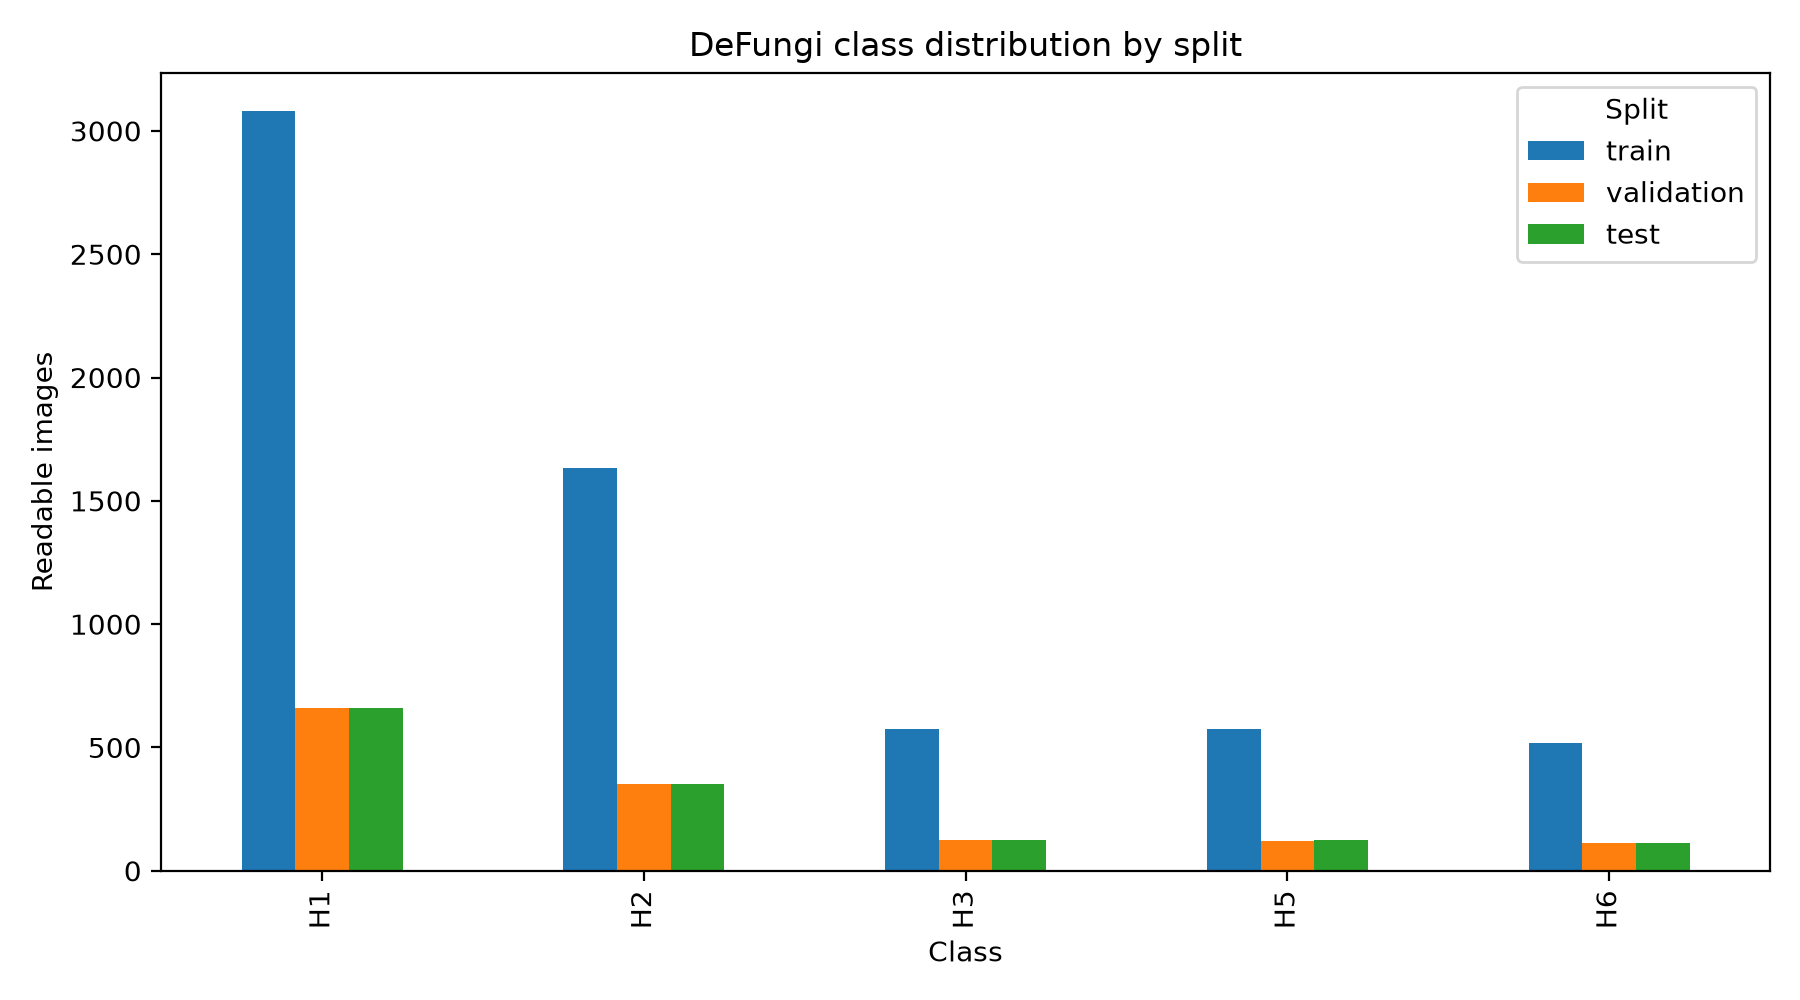
\includegraphics[width=0.72\linewidth]{figures/class_distribution.png}
\caption{Class distribution of the verified DeFungi dataset.}
\label{fig:class_distribution}
\end{figure}

The data split was created once and reused for all experiments. A stratified 70/15/15 target split was used with seed 42, giving 6,379 training images, 1,367 validation images, and 1,368 test images. The class membership of the validation and test sets is therefore fixed across custom and pretrained models.

\begin{table}[H]
\centering
\caption{Verified stratified split counts.}
\label{tab:split_counts}
\begin{tabular}{lrrrrrr}
\toprule
Split & H1 & H2 & H3 & H5 & H6 & Total \\
\midrule
Train & 3,082 & 1,634 & 573 & 573 & 517 & 6,379 \\
Validation & 661 & 350 & 123 & 122 & 111 & 1,367 \\
Test & 661 & 350 & 123 & 123 & 111 & 1,368 \\
\bottomrule
\end{tabular}
\end{table}

For the custom CNNs, all images were resized to $64 \times 64 \times 3$ and pixel values were normalized to the range $[0,1]$. For the pretrained models, images were resized to $224 \times 224 \times 3$ and processed with the corresponding Keras application preprocessing functions.

\section{Model A: Baseline CNN}
\textbf{Owner: Rifnaz.K.R.M -- 230550P}

Model A is a conventional CNN baseline using three standard convolutional layers followed by global average pooling and a small dense classifier. ReLU was used after the hidden convolutional and dense layers because it provides a simple non-linearity while avoiding saturation for positive activations. The final Softmax layer produces a probability distribution over the five fungi classes.

\begin{table}[H]
\centering
\caption{Model A architecture and parameter count.}
\label{tab:model_a_arch}
\small
\begin{tabularx}{\linewidth}{l l l r l r}
\toprule
Layer & Output Shape & Kernel & Filters/Units & Activation & Parameters \\
\midrule
Input & $64\times64\times3$ & -- & -- & -- & 0 \\
Conv2D & $64\times64\times32$ & $3\times3$ & 32 & ReLU & 896 \\
MaxPool2D & $32\times32\times32$ & $2\times2$ & -- & -- & 0 \\
Conv2D & $32\times32\times64$ & $3\times3$ & 64 & ReLU & 18,496 \\
MaxPool2D & $16\times16\times64$ & $2\times2$ & -- & -- & 0 \\
Conv2D & $16\times16\times128$ & $3\times3$ & 128 & ReLU & 73,856 \\
MaxPool2D & $8\times8\times128$ & $2\times2$ & -- & -- & 0 \\
GlobalAveragePooling2D & 128 & -- & -- & -- & 0 \\
Dense & 64 & -- & 64 & ReLU & 8,256 \\
Dense & 5 & -- & 5 & Softmax & 325 \\
\midrule
Total & -- & -- & -- & -- & 101,829 \\
\bottomrule
\end{tabularx}
\end{table}

For a standard convolution layer, the trainable parameter count is
\begin{equation}
P_{\mathrm{conv}} = (K_hK_wC_{\mathrm{in}} + 1)C_{\mathrm{out}},
\end{equation}
where the extra 1 accounts for the bias term per output channel. The layer-wise calculations are:
\begin{align}
\mathrm{Conv1} &= (3\cdot3\cdot3 + 1)\cdot32 = 896,\\
\mathrm{Conv2} &= (3\cdot3\cdot32 + 1)\cdot64 = 18,496,\\
\mathrm{Conv3} &= (3\cdot3\cdot64 + 1)\cdot128 = 73,856,\\
\mathrm{Dense64} &= (128 + 1)\cdot64 = 8,256,\\
\mathrm{Dense5} &= (64 + 1)\cdot5 = 325.
\end{align}
The total is therefore 101,829 trainable parameters. Global average pooling was used instead of flattening to reduce the classifier size after the convolutional feature extractor.

\section{Model B: Resource-Constrained CNN}
\textbf{Owner: Panuharan.S -- 230462X}

Model B was designed to reduce the parameter count while preserving the same input resolution and output classes as Model A. It replaces standard convolutional layers with depthwise separable convolutions and uses a smaller dense layer.

\begin{table}[H]
\centering
\caption{Model B architecture and parameter count.}
\label{tab:model_b_arch}
\small
\begin{tabularx}{\linewidth}{l l l r l r}
\toprule
Layer & Output Shape & Kernel & Filters/Units & Activation & Parameters \\
\midrule
Input & $64\times64\times3$ & -- & -- & -- & 0 \\
SeparableConv2D & $64\times64\times32$ & $3\times3$ & 32 & ReLU & 155 \\
MaxPool2D & $32\times32\times32$ & $2\times2$ & -- & -- & 0 \\
SeparableConv2D & $32\times32\times64$ & $3\times3$ & 64 & ReLU & 2,400 \\
MaxPool2D & $16\times16\times64$ & $2\times2$ & -- & -- & 0 \\
SeparableConv2D & $16\times16\times96$ & $3\times3$ & 96 & ReLU & 6,816 \\
MaxPool2D & $8\times8\times96$ & $2\times2$ & -- & -- & 0 \\
GlobalAveragePooling2D & 96 & -- & -- & -- & 0 \\
Dense & 48 & -- & 48 & ReLU & 4,656 \\
Dense & 5 & -- & 5 & Softmax & 245 \\
\midrule
Total & -- & -- & -- & -- & 14,272 \\
\bottomrule
\end{tabularx}
\end{table}

For a depthwise separable convolution with bias, the parameter count is
\begin{equation}
P_{\mathrm{sep}} = K_hK_wC_{\mathrm{in}} + C_{\mathrm{in}}C_{\mathrm{out}} + C_{\mathrm{out}}.
\end{equation}
The first term is the depthwise spatial convolution, the second term is the pointwise $1\times1$ convolution, and the final term is the bias. The calculations are:
\begin{align}
\mathrm{SepConv1} &= 3\cdot3\cdot3 + 3\cdot32 + 32 = 155,\\
\mathrm{SepConv2} &= 3\cdot3\cdot32 + 32\cdot64 + 64 = 2,400,\\
\mathrm{SepConv3} &= 3\cdot3\cdot64 + 64\cdot96 + 96 = 6,816,\\
\mathrm{Dense48} &= (96 + 1)\cdot48 = 4,656,\\
\mathrm{Dense5} &= (48 + 1)\cdot5 = 245.
\end{align}

Model B has 14,272 trainable parameters, which is below the 100,000-parameter target. Its FP32 parameter storage is 55.75 KB. Compared with Model A, it removes 87,557 parameters, a reduction of about 85.98\%.

\section{Optimizer Comparison}
\textbf{Owner: Peranavan.K -- 230474K}

The optimizer comparison used Model A in a controlled limited-training-batch experiment. Each optimizer was trained for 5 epochs using 30 training batches per epoch, while evaluation used the full validation split. The optimizer was selected by the lowest final validation loss, and the selected optimizer was then used for the full custom-model training runs.

\begin{table}[H]
\centering
\caption{Controlled optimizer comparison.}
\label{tab:optimizer}
\begin{tabular}{lrrrr}
\toprule
Optimizer & Learning Rate & Momentum & Final Val. Accuracy & Final Val. Loss \\
\midrule
Adam & 0.001 & 0.0 & 0.5091 & 1.2509 \\
SGD & 0.010 & 0.0 & 0.4835 & 1.4039 \\
SGD + Momentum & 0.010 & 0.9 & 0.4835 & 1.3385 \\
\bottomrule
\end{tabular}
\end{table}

Momentum updates maintain a velocity term:
\begin{align}
v_t &= \beta v_{t-1} + g_t,\\
\theta_t &= \theta_{t-1} - \eta v_t,
\end{align}
where $g_t$ is the current gradient, $\eta$ is the learning rate, and $\beta$ is the momentum coefficient. In this controlled comparison, Adam with learning rate 0.001 achieved the lowest final validation loss of 1.2508898973464966. These values are optimizer-selection evidence only and are not the final test metrics.

\section{Custom Model Training and Evaluation}
\textbf{Owner: Peranavan.K -- 230474K}

Both custom CNNs were trained using the same split and training configuration: 20 epochs, batch size 32, Adam optimizer with learning rate 0.001, and sparse categorical crossentropy. The experiments were run in a CPU-only TensorFlow environment. Test-set evaluation reports accuracy, macro precision, macro recall, macro F1-score, and confusion matrices.

\begin{figure}[H]
\centering
\begin{subfigure}{0.48\linewidth}
\centering
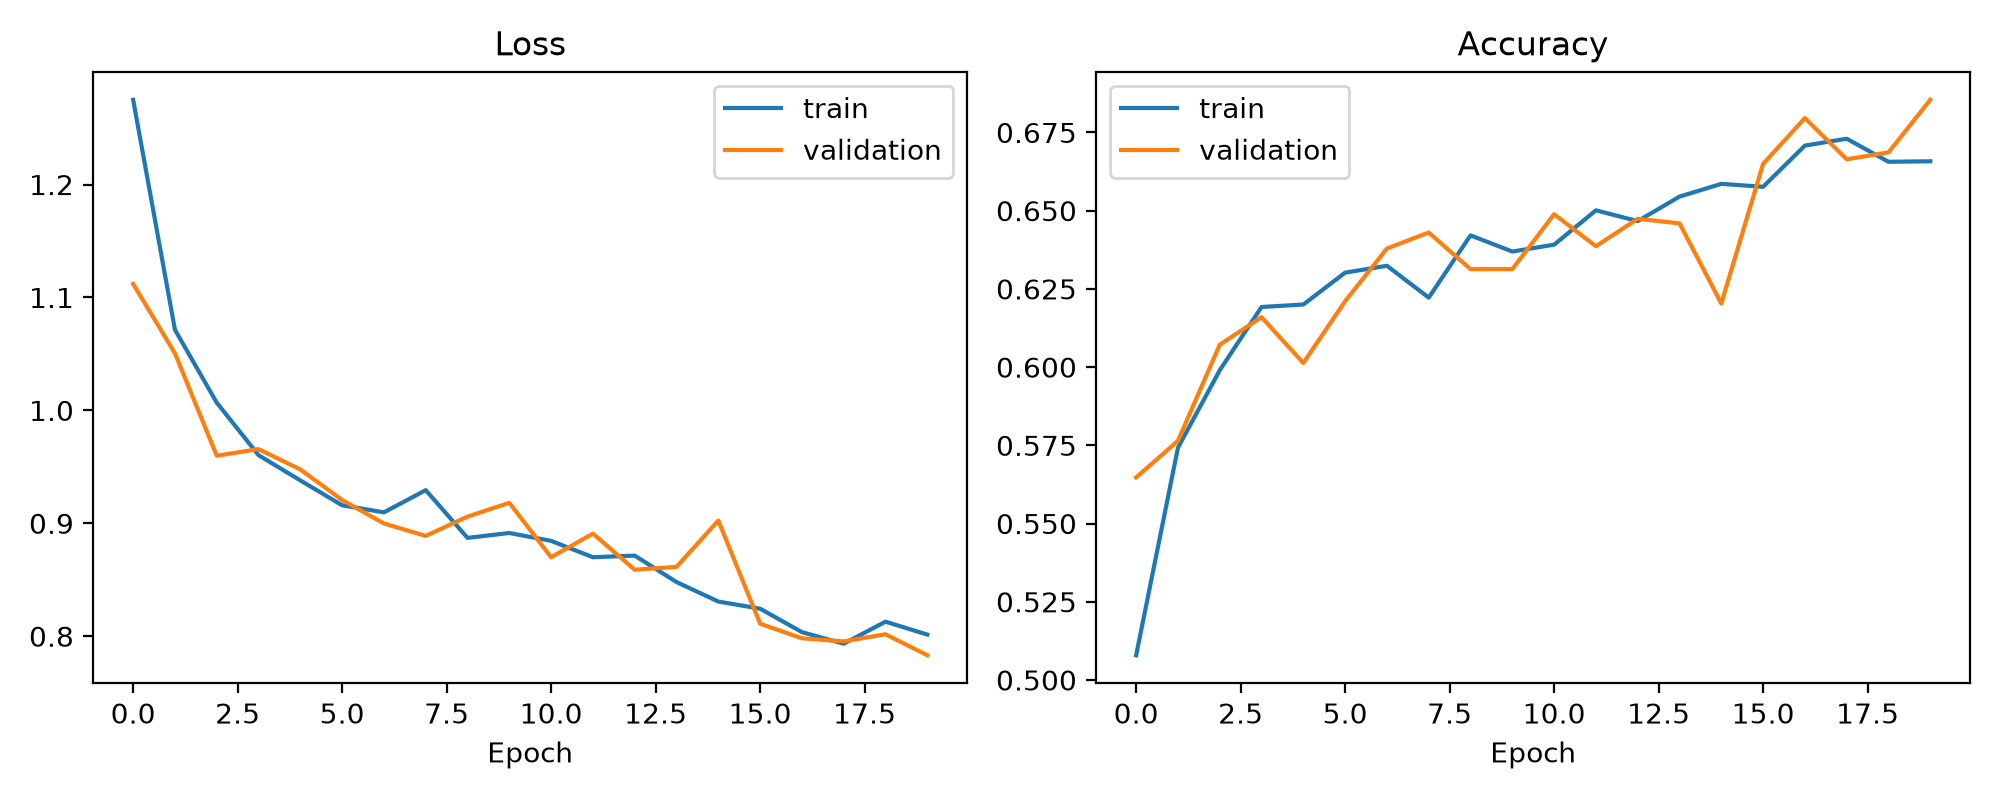
\includegraphics[width=\linewidth]{figures/model_a_history.png}
\caption{Model A learning curves.}
\label{fig:model_a_history}
\end{subfigure}
\hfill
\begin{subfigure}{0.48\linewidth}
\centering
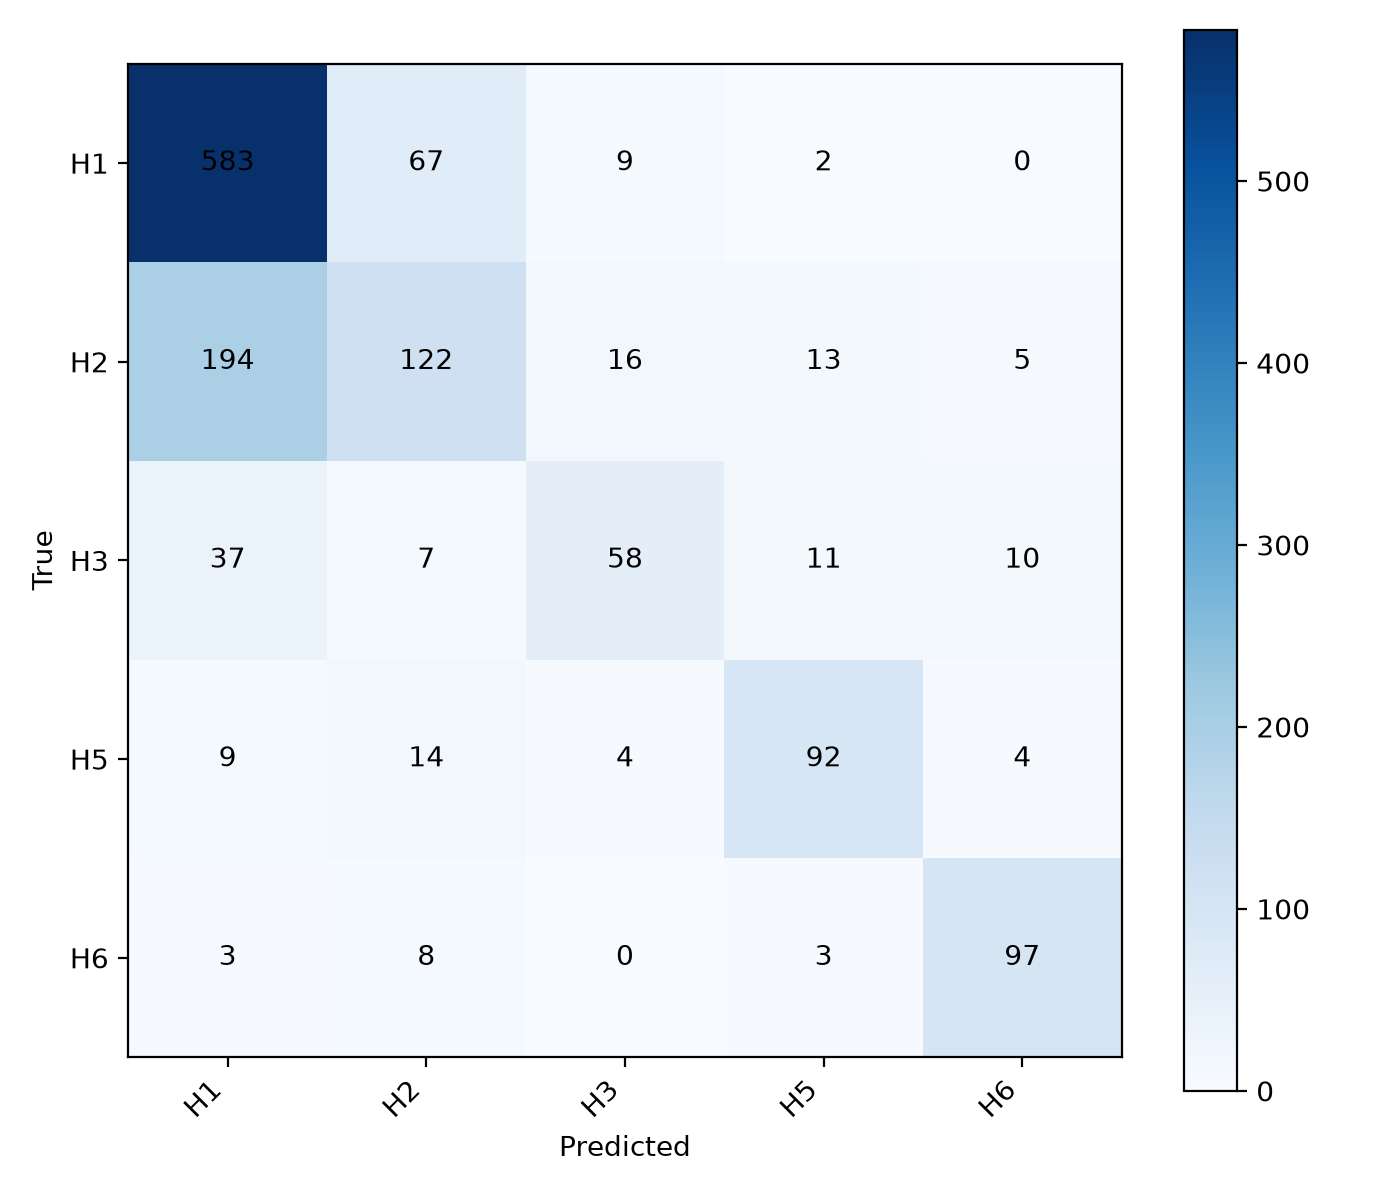
\includegraphics[width=\linewidth]{figures/model_a_confusion_matrix.png}
\caption{Model A confusion matrix.}
\label{fig:model_a_confusion}
\end{subfigure}
\caption{Model A training and test evaluation.}
\end{figure}

\begin{figure}[H]
\centering
\begin{subfigure}{0.48\linewidth}
\centering
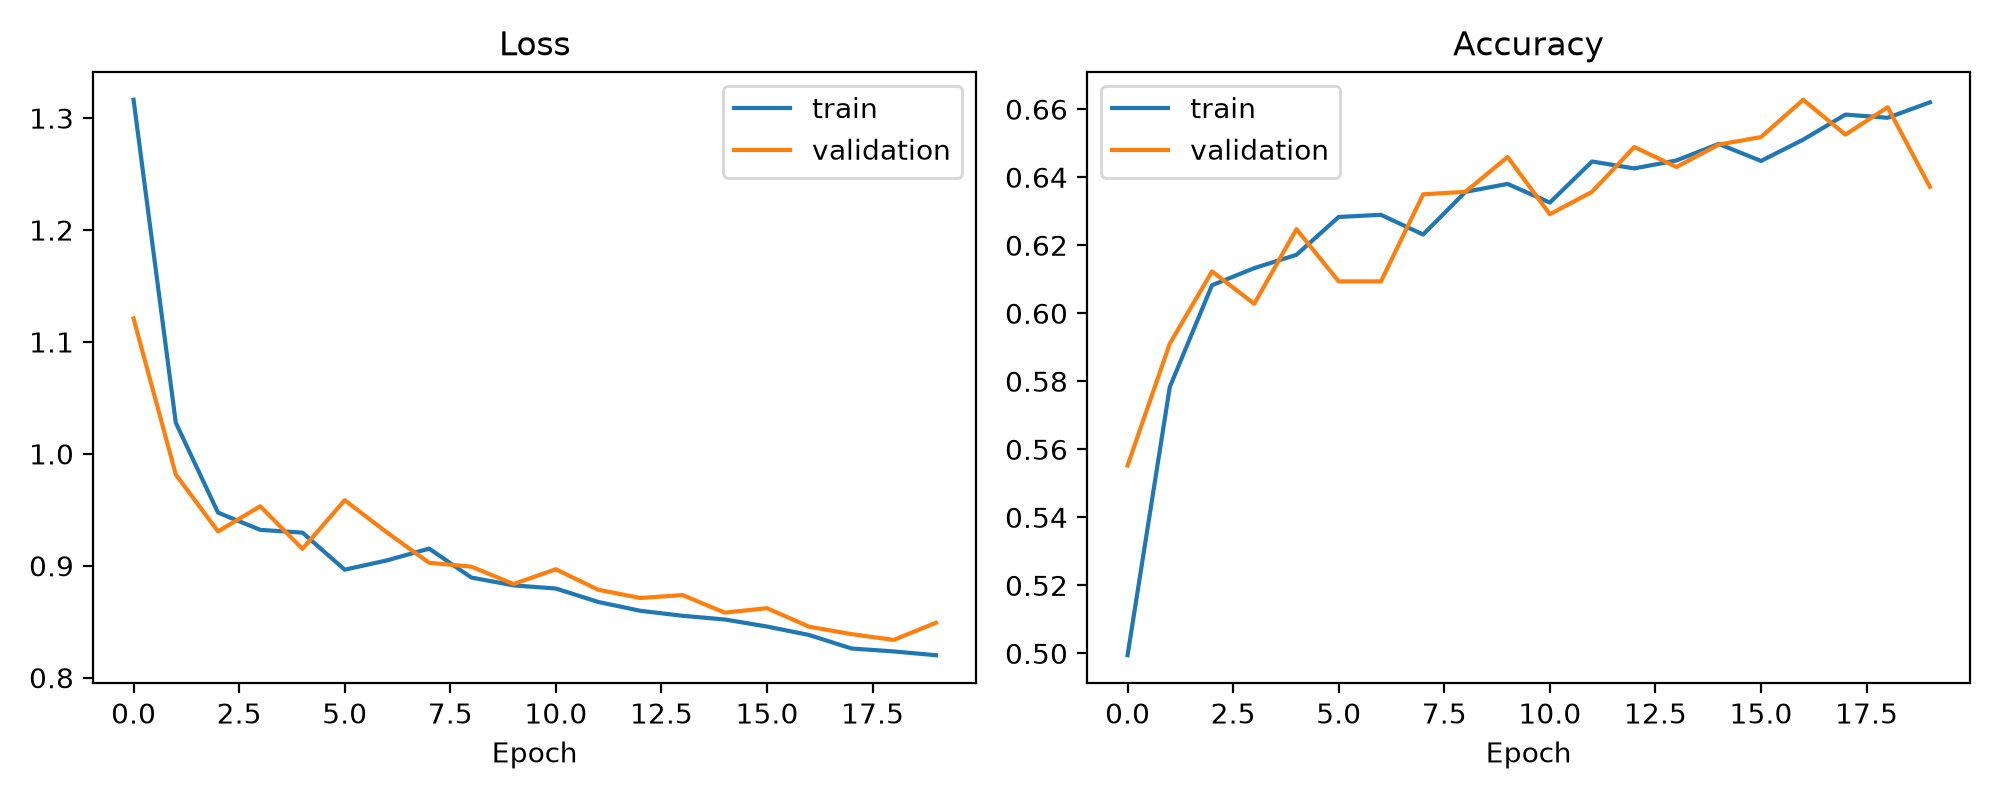
\includegraphics[width=\linewidth]{figures/model_b_history.png}
\caption{Model B learning curves.}
\label{fig:model_b_history}
\end{subfigure}
\hfill
\begin{subfigure}{0.48\linewidth}
\centering
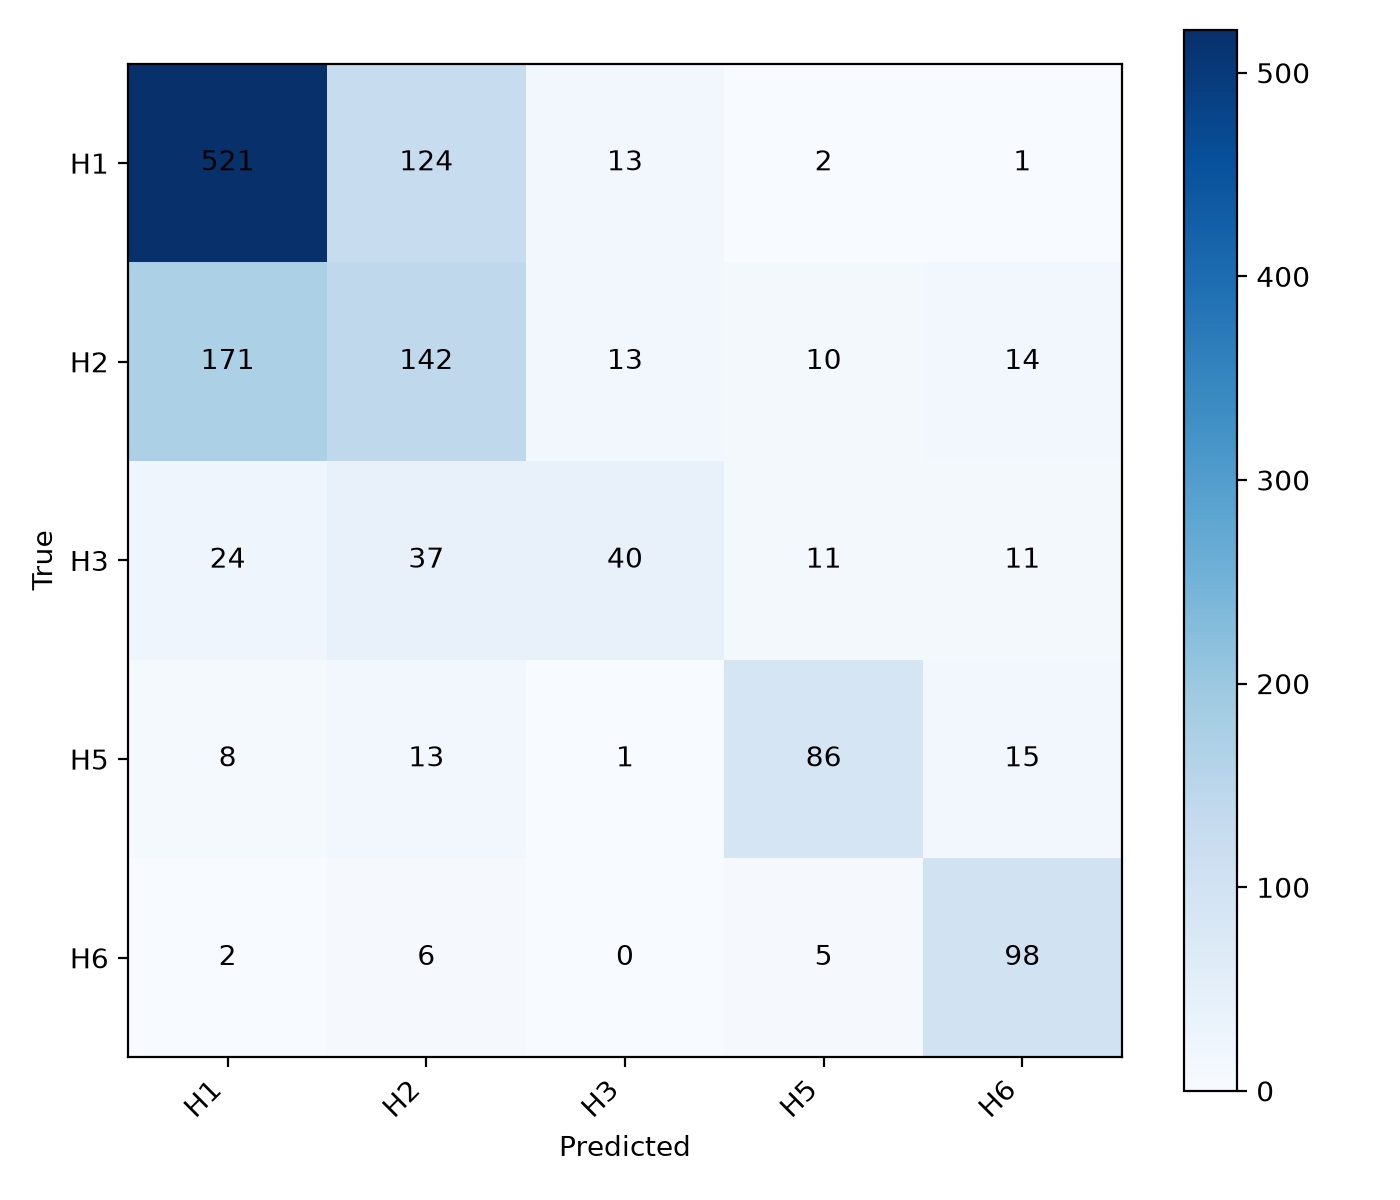
\includegraphics[width=\linewidth]{figures/model_b_confusion_matrix.png}
\caption{Model B confusion matrix.}
\label{fig:model_b_confusion}
\end{subfigure}
\caption{Model B training and test evaluation.}
\end{figure}

\begin{table}[H]
\centering
\caption{Custom CNN test-set comparison.}
\label{tab:custom_results}
\begin{tabular}{lrr}
\toprule
Metric & Model A & Model B \\
\midrule
Test accuracy & 0.6959 & 0.6484 \\
Macro precision & 0.7057 & 0.6430 \\
Macro recall & 0.6648 & 0.6202 \\
Macro F1-score & 0.6750 & 0.6209 \\
Parameters & 101,829 & 14,272 \\
FP32 parameter storage & 397.77 KB & 55.75 KB \\
Mean epoch time & 12.8958 s & 7.8730 s \\
\bottomrule
\end{tabular}
\end{table}

Model A gives higher classification performance, reaching 0.6959 test accuracy and 0.7057 macro precision. Model B trades away some accuracy for a much smaller footprint: it uses only 14,272 parameters and trains faster per epoch. This makes Model B the stronger candidate when memory and compute are the primary constraints.

\section{Pretrained Lightweight Models}
\textbf{Owner: Lavanathan.J -- 230371R}

Two lightweight ImageNet-initialized architectures were evaluated using transfer learning. In both cases, the pretrained backbone was frozen and only a new classification head was trained. The head consisted of global average pooling, dropout with rate 0.2, and a five-unit Softmax classifier. No backbone fine-tuning or unfreezing was performed.

\subsection{MobileNetV2}

MobileNetV2 is designed for efficient visual recognition using inverted residual blocks and linear bottlenecks \cite{mobilenetv2}. The model was trained with $224\times224\times3$ inputs and MobileNetV2 preprocessing.

\begin{figure}[H]
\centering
\begin{subfigure}{0.48\linewidth}
\centering
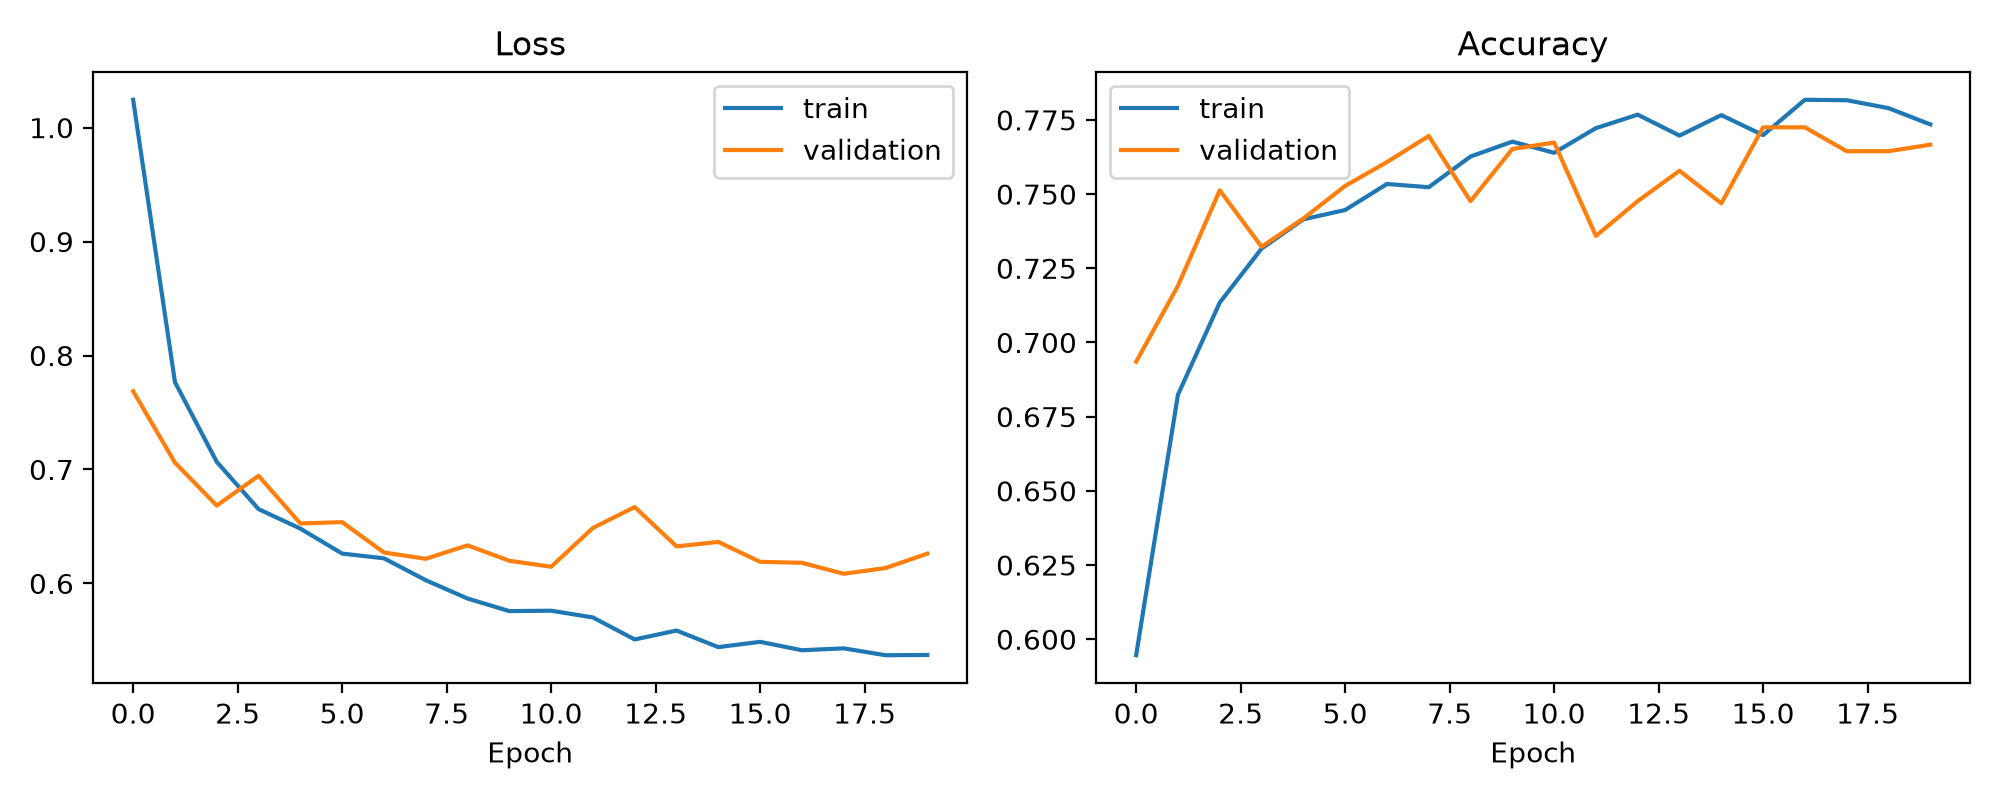
\includegraphics[width=\linewidth]{figures/mobilenetv2_history.png}
\caption{MobileNetV2 learning curves.}
\label{fig:mobilenet_history}
\end{subfigure}
\hfill
\begin{subfigure}{0.48\linewidth}
\centering
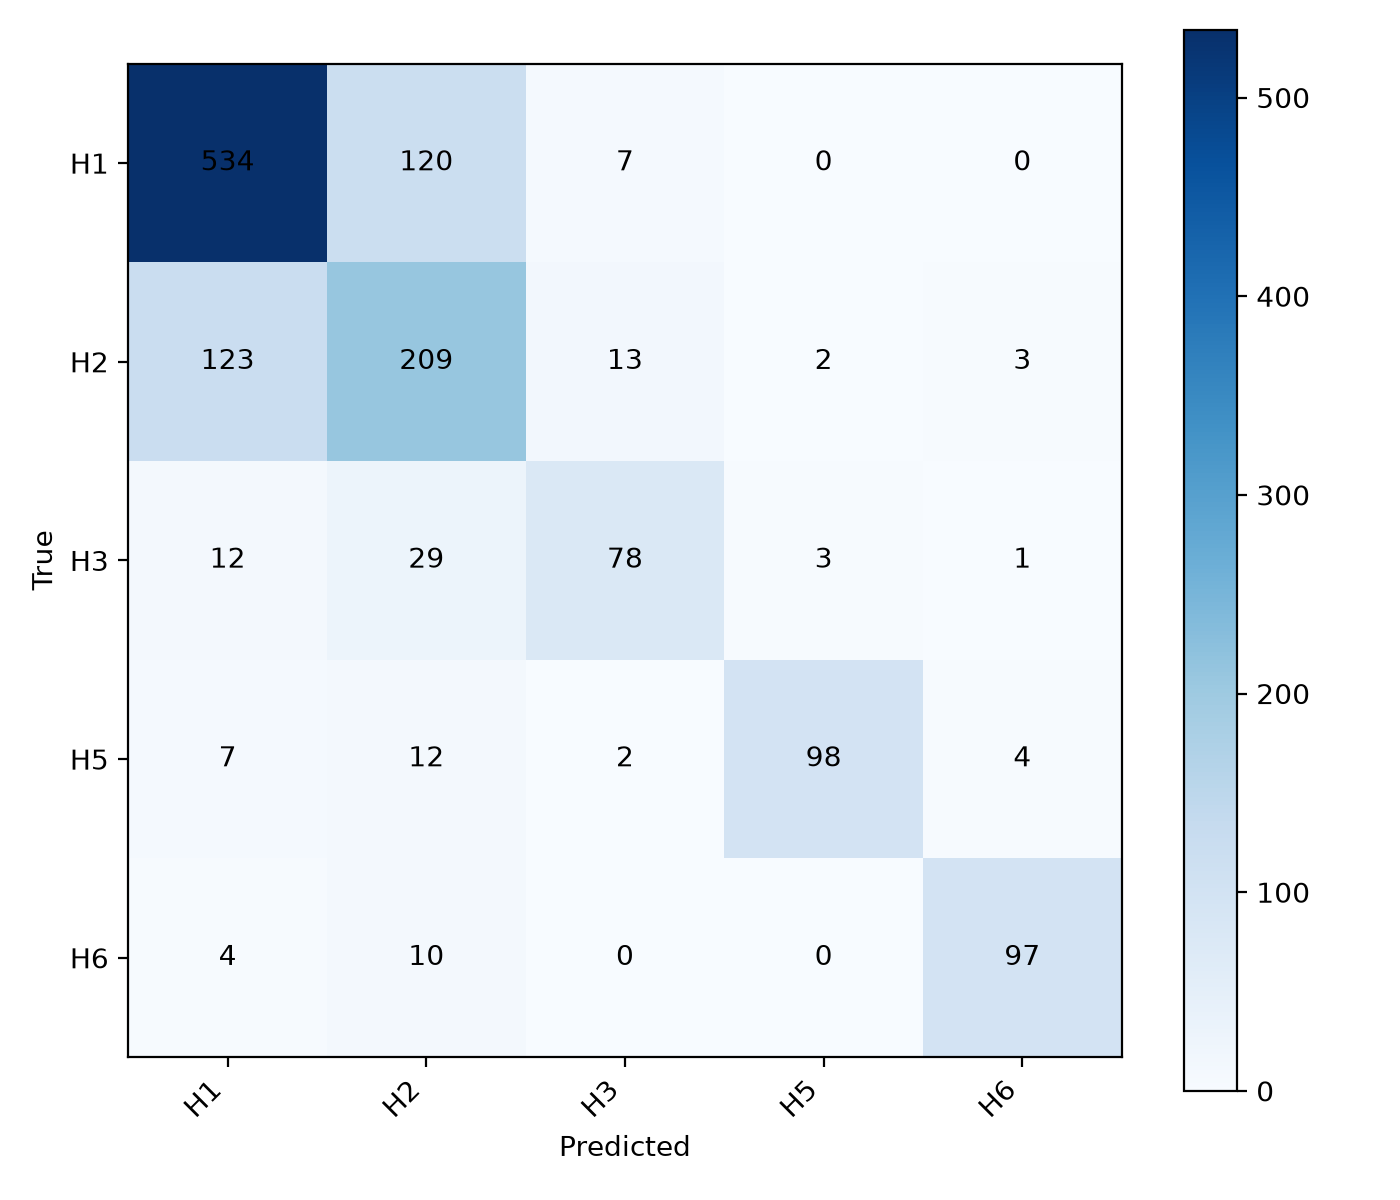
\includegraphics[width=\linewidth]{figures/mobilenetv2_confusion_matrix.png}
\caption{MobileNetV2 confusion matrix.}
\label{fig:mobilenet_confusion}
\end{subfigure}
\caption{MobileNetV2 transfer-learning evaluation.}
\end{figure}

\begin{table}[H]
\centering
\caption{MobileNetV2 results.}
\label{tab:mobilenet_results}
\begin{tabular}{lr}
\toprule
Metric & Value \\
\midrule
Total parameters & 2,264,389 \\
Trainable parameters & 6,405 \\
Saved model size & 9.25 MB \\
Mean epoch time & 100.5135 s \\
Test accuracy & 0.7427 \\
Macro precision & 0.7981 \\
Macro recall & 0.7420 \\
Macro F1-score & 0.7668 \\
\bottomrule
\end{tabular}
\end{table}

\subsection{EfficientNetB0}

EfficientNet uses compound scaling to balance network width, depth, and input resolution \cite{efficientnet}. EfficientNetB0 was trained with $224\times224\times3$ inputs and EfficientNet preprocessing.

\begin{figure}[H]
\centering
\begin{subfigure}{0.48\linewidth}
\centering
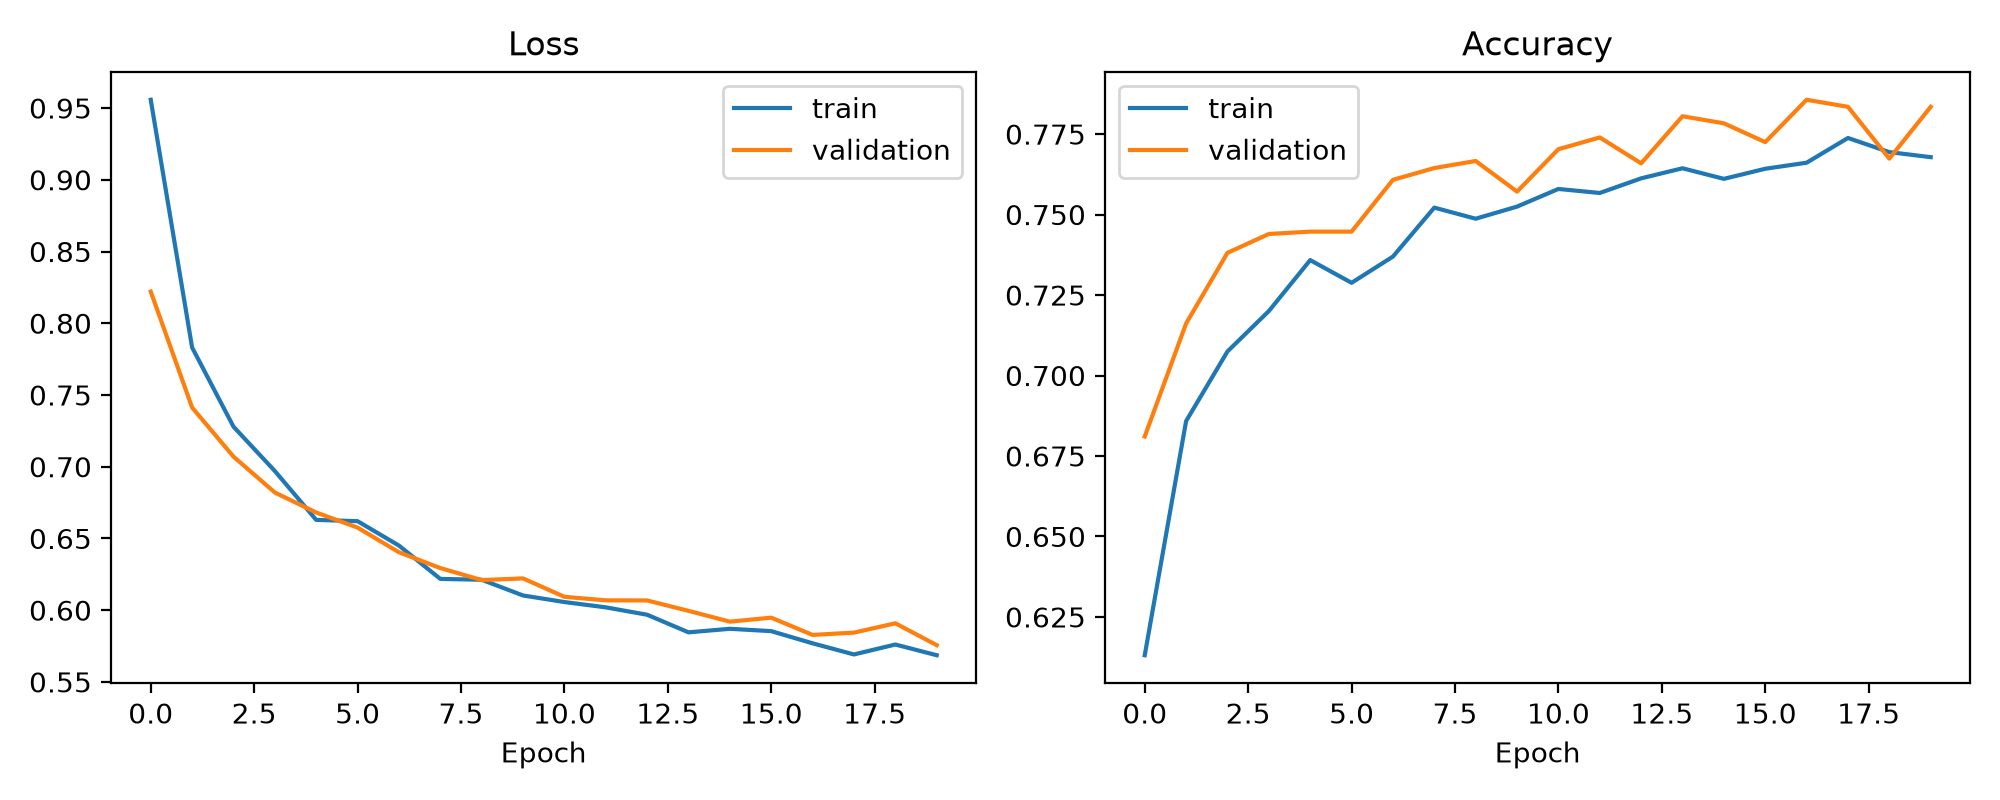
\includegraphics[width=\linewidth]{figures/efficientnetb0_history.png}
\caption{EfficientNetB0 learning curves.}
\label{fig:efficientnet_history}
\end{subfigure}
\hfill
\begin{subfigure}{0.48\linewidth}
\centering
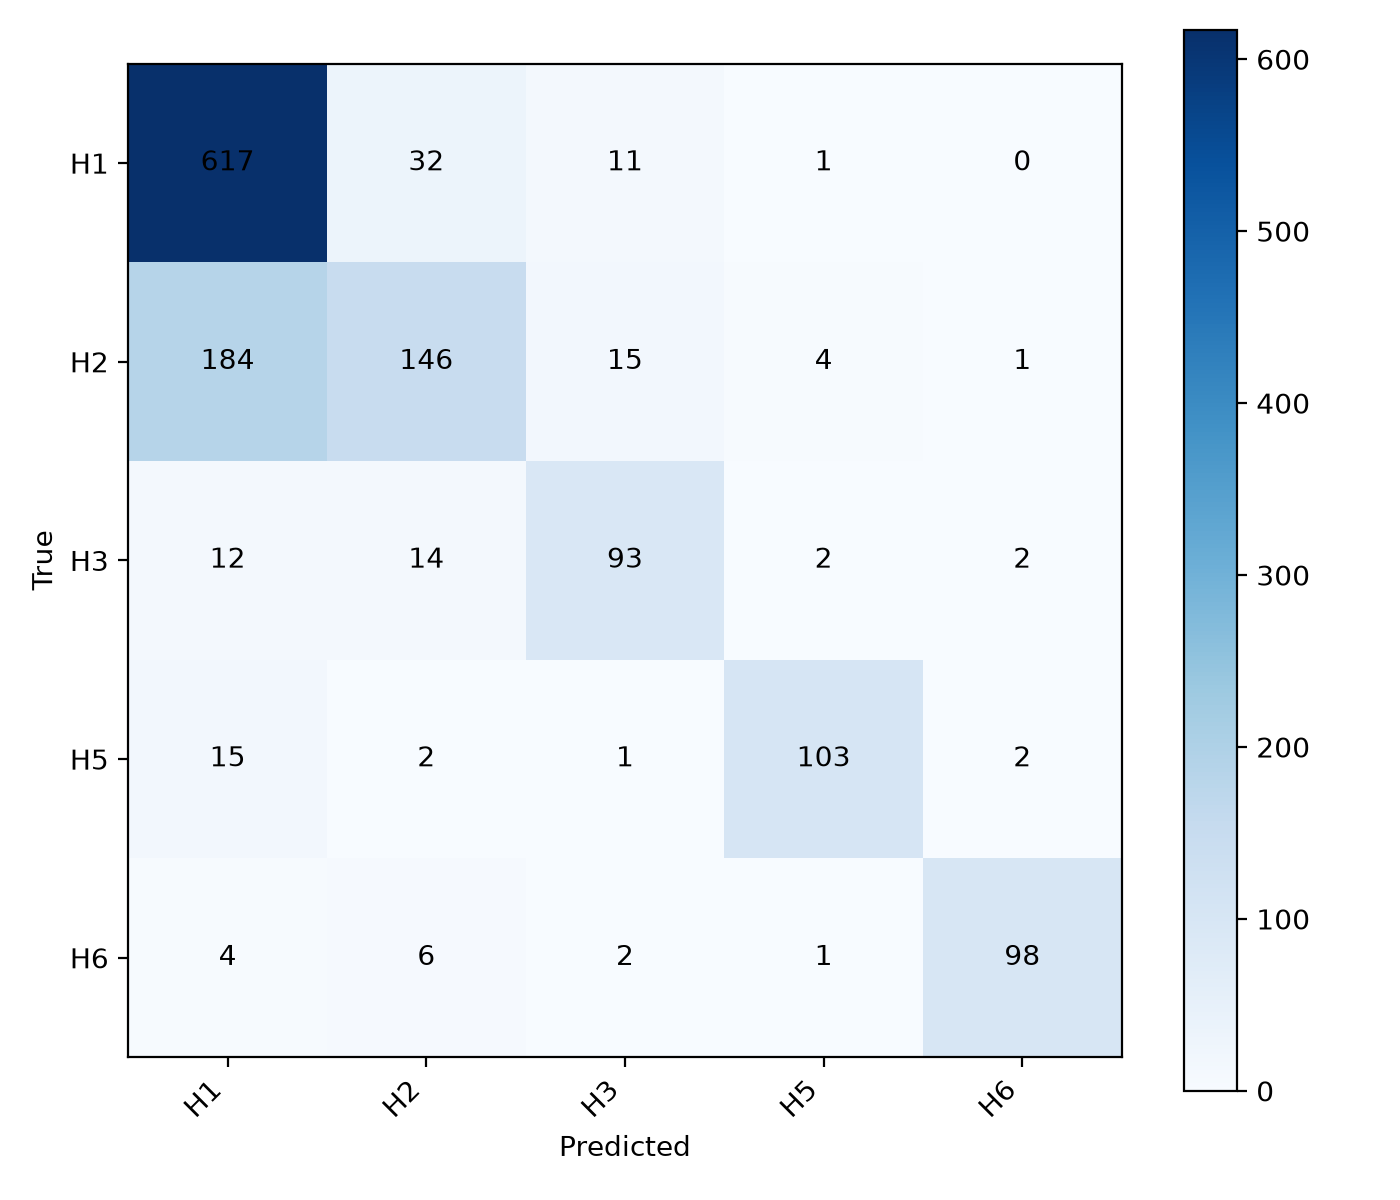
\includegraphics[width=\linewidth]{figures/efficientnetb0_confusion_matrix.png}
\caption{EfficientNetB0 confusion matrix.}
\label{fig:efficientnet_confusion}
\end{subfigure}
\caption{EfficientNetB0 transfer-learning evaluation.}
\end{figure}

\begin{table}[H]
\centering
\caption{EfficientNetB0 results.}
\label{tab:efficientnet_results}
\begin{tabular}{lr}
\toprule
Metric & Value \\
\midrule
Total parameters & 4,055,976 \\
Trainable parameters & 6,405 \\
Saved model size & 16.33 MB \\
Mean epoch time & 158.3490 s \\
Test accuracy & 0.7727 \\
Macro precision & 0.8227 \\
Macro recall & 0.7654 \\
Macro F1-score & 0.7826 \\
\bottomrule
\end{tabular}
\end{table}

\section{Final Model Comparison}
\textbf{Owner: Lavanathan.J -- 230371R}

The final comparison uses the verified `results/tables/final_comparison.csv` evidence. It compares both custom CNNs with the two Session 3 transfer-learning models. Serialized size is reported in KiB, and CPU latency is measured as batch-1 forward-pass latency on the local CPU using in-memory tensors.

\begin{table}[H]
\centering
\caption{Final verified comparison across all evaluated models.}
\label{tab:final_comparison}
\small
\begin{tabularx}{\linewidth}{lrrrr}
\toprule
Model & Accuracy & Parameters & Size (KiB) & CPU mean (ms) \\
\midrule
Model A & 0.6959 & 101,829 & 1,241.37 & 2.8241 \\
Model B & 0.6484 & 14,272 & 219.41 & 1.5922 \\
MobileNetV2 & 0.6908 & 2,264,389 & 22,000.13 & 170.1065 \\
EfficientNet-B0 & 0.7668 & 4,055,976 & 32,650.04 & 322.2855 \\
\bottomrule
\end{tabularx}
\end{table}

EfficientNet-B0 achieved the highest measured accuracy and macro recall, but it also had the largest serialized footprint and highest measured CPU latency. Model B had the smallest parameter count, smallest serialized artifact, lowest included MAC estimate, and lowest measured CPU latency. MobileNetV2 had fewer included MACs than Model A but much higher measured CPU latency on this machine, showing that parameter count and MACs alone do not establish edge performance.

\section{Conclusion}

This project completed a resource-constrained image classification pipeline on the verified DeFungi dataset. The custom baseline Model A achieved 0.6959 test accuracy with 101,829 parameters, while the compact Model B reduced the parameter count to 14,272 and FP32 parameter storage to 55.75 KB, at a lower test accuracy of 0.6484. The optimizer comparison selected Adam with learning rate 0.001 based on the lowest final validation loss in the controlled optimizer experiment.

The pretrained models were evaluated on the same split membership using the final Session 3 transfer-learning setup. MobileNetV2 reached 0.6908 test accuracy, and EfficientNet-B0 reached the best overall test accuracy of 0.7668. However, both pretrained models require substantially larger serialized model storage and higher measured CPU latency than Model B. The final results show the expected trade-off between compact custom models for edge deployment and pretrained models for stronger accuracy.

\begin{table}[H]
\centering
\caption{Member contributions.}
\label{tab:member_contributions}
\begin{tabularx}{\linewidth}{lll}
\toprule
Member & Registration Number & Contribution \\
\midrule
Rifnaz.K.R.M & 230550P & Dataset Preparation + Model A \\
Panuharan.S & 230462X & Model B + Efficiency Analysis \\
Peranavan.K & 230474K & Optimizer Comparison + Training/Evaluation \\
Lavanathan.J & 230371R & Pretrained Lightweight Models + Final Comparison \\
\bottomrule
\end{tabularx}
\end{table}


\bibliographystyle{plainnat}
\bibliography{references}

\end{document}
